\documentclass[11pt, a4paper, twoside, openright]{article} 

\usepackage{graphicx,color}
\usepackage{amssymb, amsmath, array, cite, float, url}



\begin{document}

% Example of title page for the projects carried out within DEDIS
% Copied from lasec 

% Simply include it in your mastex tex file: 
%        % Example of title page for the projects carried out within DEDIS
% Copied from lasec 

% Simply include it in your mastex tex file: 
%        % Example of title page for the projects carried out within DEDIS
% Copied from lasec 

% Simply include it in your mastex tex file: 
%        \input{cover}


% Updated October 2016


\newcommand{\logoepfl}[0]{
  \begin{center}
    
\includegraphics[width=4cm]{logo_epfl_coul.eps}
  \end{center}
  \vspace{0.3cm}
  \hrule
}
\newcommand{\project}[1]{
  \begin{center}
    \large{#1}
  \end{center}
  \vspace{1cm}
}
\newcommand{\department}[1]{
  \begin{center}
    \large{#1}
  \end{center}
}
\newcommand{\lab}[1]{
  \begin{center}
    \large{#1}
  \end{center}
}
\newcommand{\supervisor}[3]{
  \begin{center}
    \begin{normalsize}{
        \bf #1}\\#2\\#3
    \end{normalsize}
  \end{center}
}
\renewcommand{\author}[1]{
  \begin{center}
    \Large{#1}
  \end{center}
  \vspace{0.5cm}
}
\renewcommand{\title}[1]{
  \vspace{3cm}
  \begin{center}
    \huge{#1}
  \end{center}
  \vspace{1.7cm}
}
\renewcommand{\date}[2]{
  \begin{center}
    \normalsize{#1 #2}
  \end{center}
  \vspace{0.5cm}
}


\thispagestyle{empty}


% begin title page
  \logoepfl
  
  \title{WebAssembly Execution Environment for Dela
}
  
  \author{Maxime Sierro}
  \department{School of Computer and Communication Sciences}
  \lab{Decentralized and Distributed Systems lab}
  \project{Master Semester Project}
  
  \date{June}{2021}

  \begin{center}
    \begin{tabular}{cc}
      \begin{tabular}{p{4.0cm}}
        \supervisor{Responsible}{Prof. Bryan Ford}{EPFL / DEDIS}
      \end{tabular}&
      \begin{tabular}{p{4.0cm}}
        \supervisor{Supervisor}{Noémien Kocher}{EPFL / DEDIS}
      \end{tabular}
    \end{tabular}
  \end{center}

% end title page




% Updated October 2016


\newcommand{\logoepfl}[0]{
  \begin{center}
    
\includegraphics[width=4cm]{logo_epfl_coul.eps}
  \end{center}
  \vspace{0.3cm}
  \hrule
}
\newcommand{\project}[1]{
  \begin{center}
    \large{#1}
  \end{center}
  \vspace{1cm}
}
\newcommand{\department}[1]{
  \begin{center}
    \large{#1}
  \end{center}
}
\newcommand{\lab}[1]{
  \begin{center}
    \large{#1}
  \end{center}
}
\newcommand{\supervisor}[3]{
  \begin{center}
    \begin{normalsize}{
        \bf #1}\\#2\\#3
    \end{normalsize}
  \end{center}
}
\renewcommand{\author}[1]{
  \begin{center}
    \Large{#1}
  \end{center}
  \vspace{0.5cm}
}
\renewcommand{\title}[1]{
  \vspace{3cm}
  \begin{center}
    \huge{#1}
  \end{center}
  \vspace{1.7cm}
}
\renewcommand{\date}[2]{
  \begin{center}
    \normalsize{#1 #2}
  \end{center}
  \vspace{0.5cm}
}


\thispagestyle{empty}


% begin title page
  \logoepfl
  
  \title{WebAssembly Execution Environment for Dela
}
  
  \author{Maxime Sierro}
  \department{School of Computer and Communication Sciences}
  \lab{Decentralized and Distributed Systems lab}
  \project{Master Semester Project}
  
  \date{June}{2021}

  \begin{center}
    \begin{tabular}{cc}
      \begin{tabular}{p{4.0cm}}
        \supervisor{Responsible}{Prof. Bryan Ford}{EPFL / DEDIS}
      \end{tabular}&
      \begin{tabular}{p{4.0cm}}
        \supervisor{Supervisor}{Noémien Kocher}{EPFL / DEDIS}
      \end{tabular}
    \end{tabular}
  \end{center}

% end title page




% Updated October 2016


\newcommand{\logoepfl}[0]{
  \begin{center}
    
\includegraphics[width=4cm]{logo_epfl_coul.eps}
  \end{center}
  \vspace{0.3cm}
  \hrule
}
\newcommand{\project}[1]{
  \begin{center}
    \large{#1}
  \end{center}
  \vspace{1cm}
}
\newcommand{\department}[1]{
  \begin{center}
    \large{#1}
  \end{center}
}
\newcommand{\lab}[1]{
  \begin{center}
    \large{#1}
  \end{center}
}
\newcommand{\supervisor}[3]{
  \begin{center}
    \begin{normalsize}{
        \bf #1}\\#2\\#3
    \end{normalsize}
  \end{center}
}
\renewcommand{\author}[1]{
  \begin{center}
    \Large{#1}
  \end{center}
  \vspace{0.5cm}
}
\renewcommand{\title}[1]{
  \vspace{3cm}
  \begin{center}
    \huge{#1}
  \end{center}
  \vspace{1.7cm}
}
\renewcommand{\date}[2]{
  \begin{center}
    \normalsize{#1 #2}
  \end{center}
  \vspace{0.5cm}
}


\thispagestyle{empty}


% begin title page
  \logoepfl
  
  \title{WebAssembly Execution Environment for Dela
}
  
  \author{Maxime Sierro}
  \department{School of Computer and Communication Sciences}
  \lab{Decentralized and Distributed Systems lab}
  \project{Master Semester Project}
  
  \date{June}{2021}

  \begin{center}
    \begin{tabular}{cc}
      \begin{tabular}{p{4.0cm}}
        \supervisor{Responsible}{Prof. Bryan Ford}{EPFL / DEDIS}
      \end{tabular}&
      \begin{tabular}{p{4.0cm}}
        \supervisor{Supervisor}{Noémien Kocher}{EPFL / DEDIS}
      \end{tabular}
    \end{tabular}
  \end{center}

% end title page



\newpage
\setcounter{page}{1}
\tableofcontents
\newpage
        

\section{Introduction}
The goal of the project is to implement a smart contract execution environment which uses WebAssembly \cite{webassembly} to handle smart contracts written in different languages. It must communicate with the DELA framework \cite{dela}, which is a blockchain-based distributed ledger currently developed in Go by the Decentralized and Distributed Systems lab.
Only a small subset of said framework must receive changes to communicate with the new environment. As a result, the vast majority of the work is focused on the environment itself, which is implemented from scratch.

\subsection{Motivation}

\begin{figure}[htbp]
 \centering
  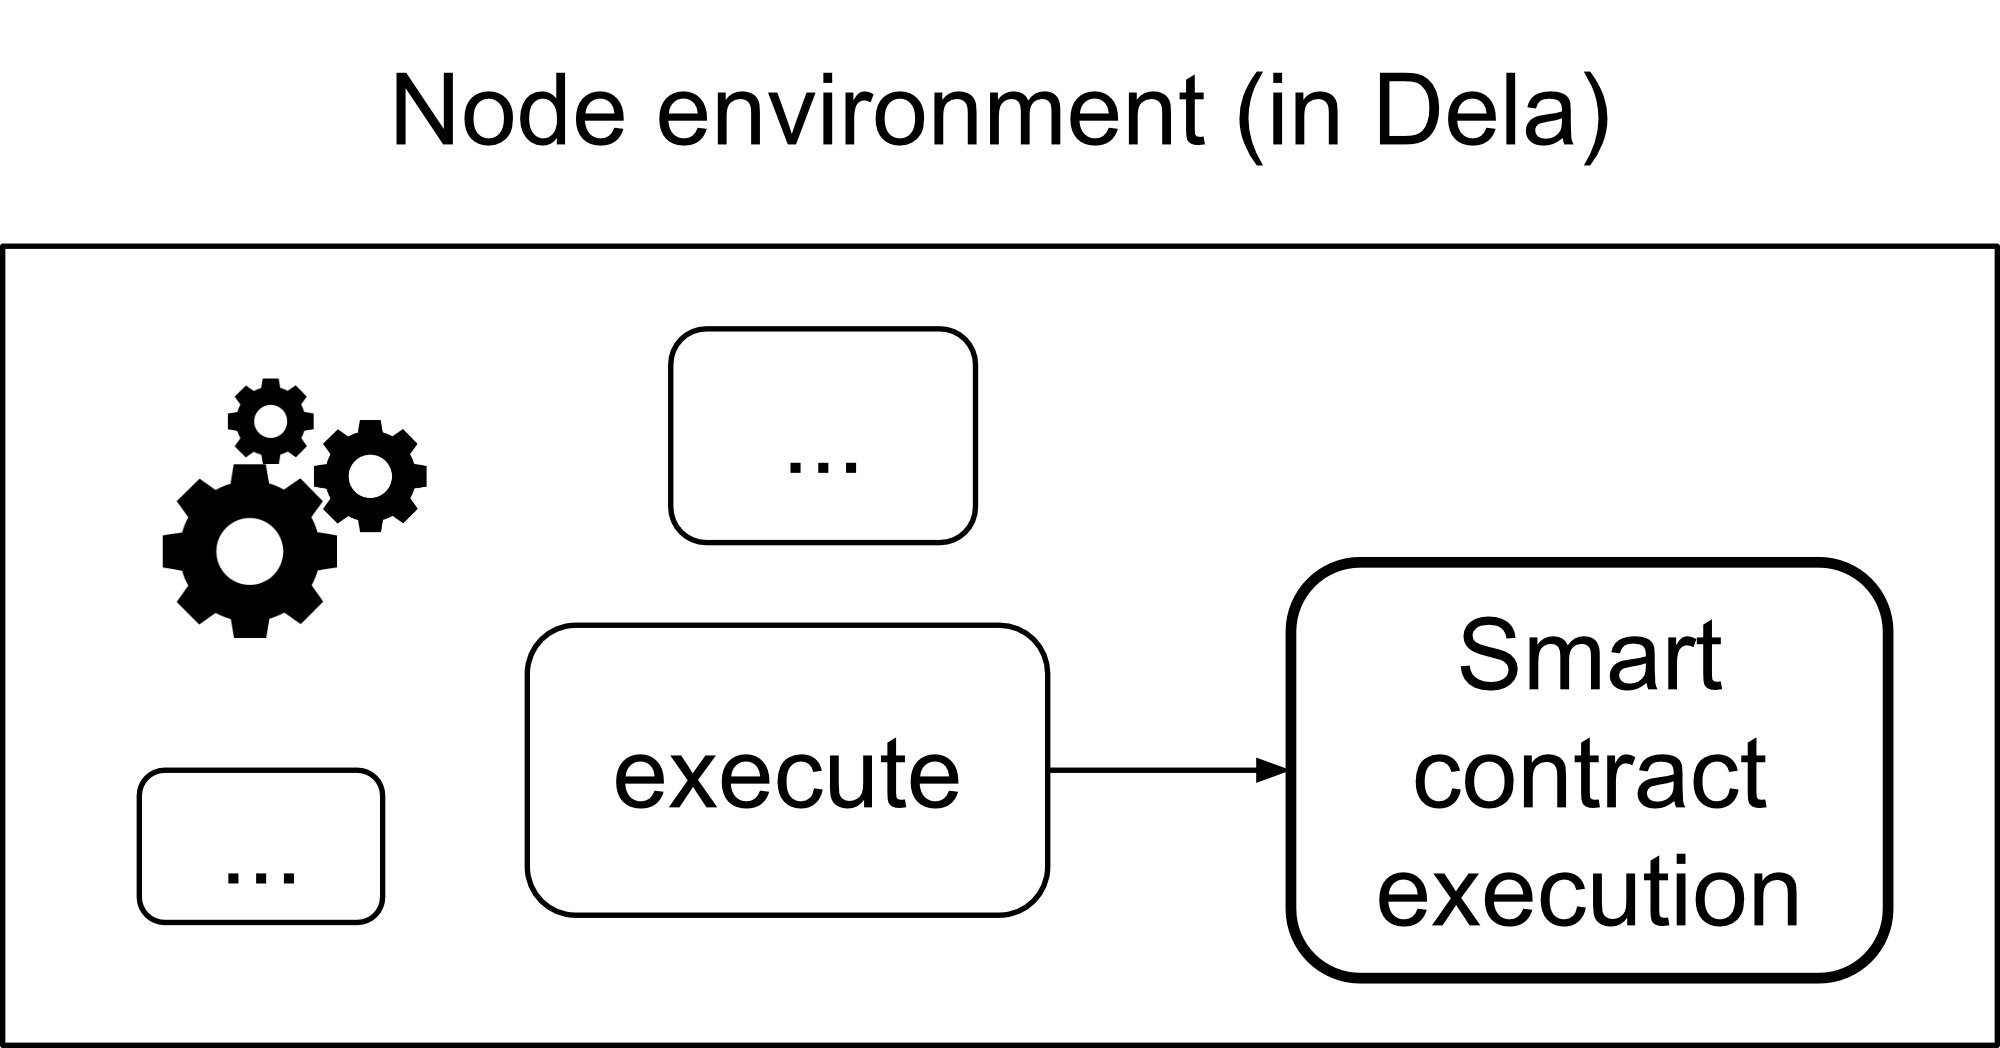
\includegraphics[width=12cm]{wasm1.png}
  \caption{Native smart contracts execution environment.}
\end{figure}


As shown in figure 1, the standard way of executing a smart contract in DELA is inside of a node's environment, which we call ``native'' execution. While this method is very intuitive and efficient, it has two main limitations. The first one is that adding, removing or modifying a smart contract requires re-compiling the entirety of the environment, which is highly unpractical in a realistic blockchain scenario where such changes are frequent. The second is that smart contracts are required to be pre-compiled for the environment running the ledger and must thus be written in the same language, which is Go in this case.

\begin{figure}[htbp]
 \centering
  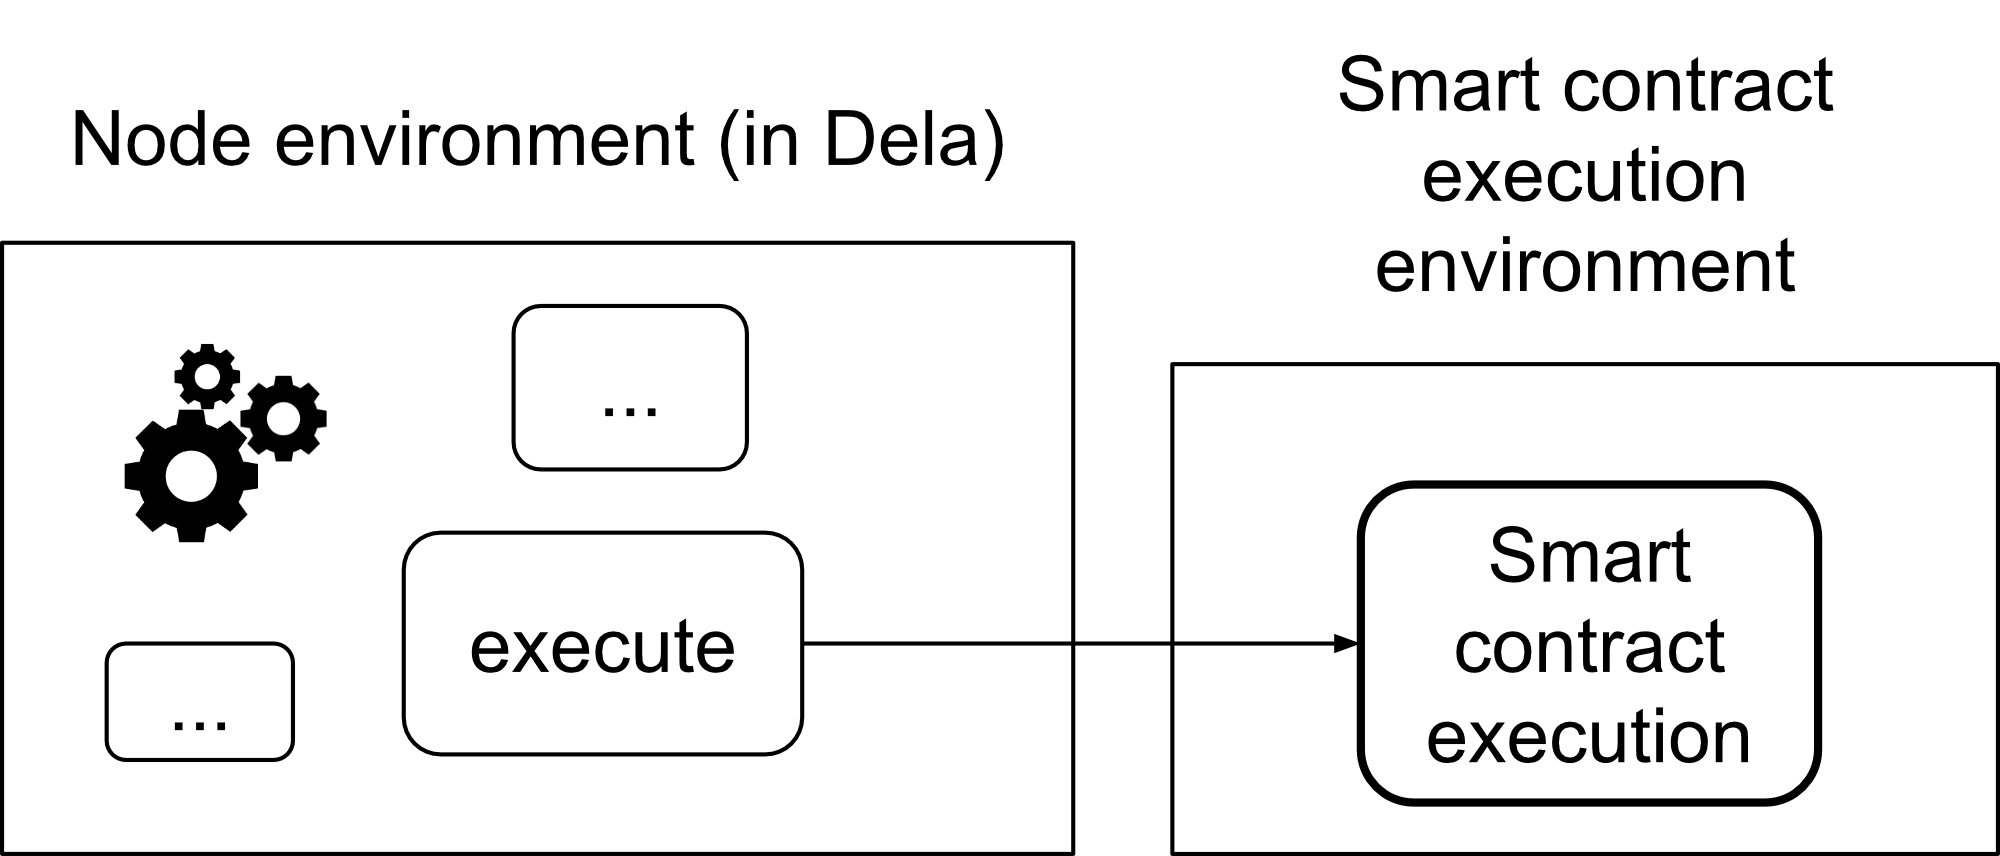
\includegraphics[width=12cm]{wasm2.png}
  \caption{Decoupled smart contracts execution environment.}
\end{figure}

To circumvent the first limitation, the obvious solution is to decouple the smart contract execution environment from the node's environment, as illustrated in figure 2. Any modification on the smart contracts would only require recompiling the smaller, decoupled environment which opens up the possibility of loading and unloading smart contracts dynamically without interrupting the main DELA environment. With this decoupled environment, smart contracts must not necessarily be written in Go, which somewhat takes care of the second limitation. However, supporting multiple languages efficiently is not straightforward and requires something else, which is when WebAssembly comes into the picture.

WebAssembly (WASM) is an open standard that defines a binary format which can obtained from higher level compatible languages. As its name implies, it is made up of ``Assembly-like'' instructions which can thus be run on a wide range of machines very efficiently, thanks to their low level. The WASM code is executed in a sandboxed environment. This added flexibility, its host independence and low performance penalty make it an ideal candidate for a smart-contract runtime used by many nodes trying to reach a consensus. Ethereum's proposed redesign of their execution layer using WASM further indicates that there is great potential for the technology in the blockchain field. 

\subsection{Goals}
\label{Goals}

\begin{enumerate} 

\itemsep0em

 \item Implementation of a fully functional execution module that uses WASM
 \item Simultaneous support of multiple smart contracts written in different languages
 \item Justification of configuration choices and the selection of compatible languages
 \item Performance comparisons
 \item Determinism analysis
 \item Testing comparable to the native module

\end{enumerate} 

\section{Design}

\subsection{General Configuration}
The most important design decision during the project was deciding what ``kind'' of environment should be built. WebAssembly was introduced in 2017, when its initial aim was to enable high performance web-browser applications. Over time however, WASM started seeing use outside of browsers because of its many advantages, especially its near-native performance and consistent execution across different hardwares. As a result, three options were identified and considered : a web browser application, a web server and a unix daemon.

The first factor that was taken into account was the general lack of resources on WASM, which is severely exacerbated when the environment is not browser-based. Even though a web-browser application functionally made less sense than the other options since there is no human interaction, it was the chosen solution at the start of the project. The daemon would have communicated with the DELA framework using unix sockets and would have used a runtime like Wasmer \cite{wasmer}, Wasmtime \cite{wasmtime} or WAVM \cite{wavm}.
\subsection{Supported Languages}


\section{Implementation}

\subsection{WebAssembly Compilation}

\subsection{Environment Setup}

\subsection{Smart Contract Execution}

\subsection{Communication with DELA}


\section{Results}

\subsection{Counter Increase}

\subsection{Generator Multiplication}

\subsection{ed25519 Point Addition}

\subsection{ed25519 Point Multiplication}

\section{Discussion}

\subsection{Determinism}

\subsection{Automated Smart Contract Loading}


\section{Future Work}

\section{Conclusion}
\newpage
\section{Bibliography}
\bibliographystyle{unsrt}
\bibliography{biblio}
\end{document}
